% Chapter 4: interpreting neural networks.
% Requires: amsmath, amssymb, bm, graphicx, booktabs, multirow, subcaption, algorithm, algpseudocode,
% tikz (arrows.meta, positioning, calc, decorations.pathreplacing, shapes.geometric, fit), natbib.
% Computed figures are produced by scripts/make_figures.py; figures/slides/ holds figures taken from the lecture slides.

\providecommand{\R}{\mathbb{R}}
\providecommand{\E}{\mathbb{E}}
\providecommand{\Normal}{\mathcal{N}}
\providecommand{\argmax}{\operatorname*{arg\,max}}
\providecommand{\argmin}{\operatorname*{arg\,min}}
\providecommand{\vy}{\mathbf{y}}
\providecommand{\vx}{\mathbf{x}}
\providecommand{\mX}{\mathbf{X}}
\providecommand{\mI}{\mathbf{I}}
\providecommand{\vb}{\boldsymbol{\beta}}
\providecommand{\veps}{\boldsymbol{\epsilon}}
\providecommand{\vp}{\mathbf{p}}
\providecommand{\vg}{\mathbf{g}}
\providecommand{\ind}{\mathbf{1}}
\providecommand{\vz}{\mathbf{z}}
\providecommand{\vh}{\mathbf{h}}
\providecommand{\vw}{\mathbf{w}}
\providecommand{\vs}{\mathbf{s}}
\providecommand{\ve}{\mathbf{e}}
\providecommand{\mW}{\mathbf{W}}
\providecommand{\relu}{\operatorname{ReLU}}
\providecommand{\IG}{\operatorname{IG}}

% TikZ styles shared by the network diagrams in this chapter
\tikzset{
  nn/.style={circle, draw, fill=blue!12, minimum size=7mm, inner sep=0pt, font=\scriptsize},
  nnr/.style={nn, fill=red!30},
  nny/.style={nn, fill=yellow!70},
  nnb/.style={draw, rectangle, minimum size=4mm, inner sep=1pt, font=\scriptsize, fill=white},
  wlab/.style={font=\tiny, fill=white, inner sep=0.6pt},
  lyr/.style={font=\scriptsize, anchor=east, text=black!70},
}

\providecommand{\chaptertoc}{}
\chapter{Interpreting neural networks}
\label{ch:interpretation}
\chaptertoc

The convolutional networks and transformers of Chapters 2 and 3 predict chromatin accessibility, transcription factor binding and gene expression from DNA sequence with high accuracy. Accuracy alone, however, is rarely the end goal in genomics. If a model predicts that a sequence is an active enhancer, we want to know \emph{why}: which nucleotides drive the prediction, which transcription factor motifs they correspond to, and how a mutation at a given position would change the output. This chapter develops methods that answer these questions for a trained network. They assign an importance score to each input feature, for example each nucleotide, for one prediction at a time. We start from the most intuitive approach, perturbing the input and observing the output, and then derive a sequence of increasingly principled methods based on backpropagation: gradients, deconvolutional networks, guided backpropagation, DeepLIFT and integrated gradients. We close with Shapley values, which provide a theoretical framework that connects several of these methods.

%======================================================================
\section{Why interpret a neural network?}
\label{sec:why_interpret}
%======================================================================

There is a broad trade-off between the predictive power of a method and how easily we can interpret it (Figure~\ref{fig:power_interp}). Classical statistical models, such as the linear and L1-regularized regression of Chapter 1, are interpretable: each feature has a coefficient, and features with large coefficients matter. Traditional machine learning methods, such as support vector machines and random forests, are often more accurate, particularly on tabular data, but are harder to interpret. Deep neural networks, which may have billions of parameters and many layer types, are typically the most accurate on sequence data, and they learn useful representations of the data that would be difficult to engineer by hand. They are also the hardest to understand, and their ``black box'' nature is a common criticism~\citep{castelvecchi2016}. Suppose we train a model to predict which DNA mutations cause a disease. If the model performs well, it has likely learned patterns that we would also like to understand. The aim of interpretation methods is to keep the power of deep learning while recovering some of the insight that simpler models give for free.

\begin{figure}[t]
  \centering
  \begin{tikzpicture}[>=Stealth, every node/.style={font=\small}]
    \draw[->, thick] (0,0) -- (7.5,0) node[below left] {interpretability};
    \draw[->, thick] (0,0) -- (0,4.2) node[above left, rotate=90, anchor=south east] {predictive power};
    \fill[blue!60!black] (1.0,3.5) circle (2.5pt) node[right] {deep learning};
    \fill[blue!60!black] (3.4,2.1) circle (2.5pt) node[right] {traditional machine learning};
    \fill[blue!60!black] (5.6,0.8) circle (2.5pt) node[above] {classical statistics};
    \draw[dashed] (1.0,3.5) -- (3.4,2.1) -- (5.6,0.8);
    \node[draw, rounded corners, fill=green!10, align=center] (goal) at (5.6,3.5) {interpretable\\deep learning};
    \draw[->, thick, green!40!black] (1.35,3.5) -- (goal.west);
  \end{tikzpicture}
  \caption{The trade-off between predictive power and interpretability. Interpretation methods aim to move deep learning models to the right without losing power.}
  \label{fig:power_interp}
\end{figure}

\subsection{What would we like to know?}

Before introducing methods, it helps to list the ways one might try to understand how a trained network makes its predictions.
\begin{itemize}
  \item \emph{Look at the learned parameters.} For a simple network this can work. The first-layer convolutional filters of the Basset model~\citep{kelley2016} (Chapter 3) resemble the position weight matrices of known transcription factor motifs. Deeper layers combine filters in ways that are much harder to read off, and even first-layer filters do not always correspond to clean motifs.
  \item \emph{Ablation.} Remove or zero out an input feature, a filter or an internal node, and measure the change in performance. Done across the whole data set this gives a \emph{global} measure of importance; done for one data point it measures how much a single prediction depends on that component. Ablation is related to stepwise regression in classical statistics: forward stepwise regression starts with no features and repeatedly adds the most useful one, while backward stepwise regression starts with all features and repeatedly removes the least useful.
  \item \emph{Attention weights.} For transformers, the attention matrices show which positions each position attends to. The Enformer model~\citep{avsec2021} was shown to attend to topologically associating domain (TAD) boundaries in this way (Chapter 3). With many layers and many heads per layer, though, the attention weights must be aggregated in some ad hoc way, typically averaged, which makes them harder to interpret.
  \item \emph{Saliency maps.} Ask how much a small change to each input feature would change the output for one data point. This can be computed by perturbation (in silico mutagenesis) or by backpropagation (gradients). It is a \emph{local} measure: it describes the model near one input.
  \item \emph{Local linearization.} We know how to interpret a linear model. Replacing the whole network by a linear model would defeat the purpose of using a network, but we can approximate it by a linear model \emph{near} a given data point and interpret that approximation. Gradients do exactly this, and we will see that several other methods can be viewed as better-behaved linearizations.
  \item \emph{Input optimization.} Find inputs that maximize or minimize the output. Unconstrained, the optimal input is often unnatural and not very informative. A more useful variant starts from a real data point and asks how it could be changed to increase or decrease the prediction.
\end{itemize}
Most of this chapter is about \emph{local feature attribution}: given a trained model and one input, assign a score to each input feature that reflects its importance for that prediction (Figure~\ref{fig:attribution_task}). Scores for many inputs can then be aggregated, for example by clustering high-scoring subsequences into motifs, to give a global picture.

\begin{figure}[t]
  \centering
  \begin{tikzpicture}[>=Stealth, every node/.style={font=\small, align=center}]
    \node[draw, minimum width=4.8cm, minimum height=0.6cm, font=\ttfamily\small] (seq) {ACGTTGATAAGCCTCAGATGGTA};
    \node[above=0.1cm of seq] {input sequence $\vx$};
    \node[draw, rounded corners, fill=blue!8, right=1.2cm of seq] (model) {trained model $f$\\(e.g.\ CNN)};
    \node[right=0.9cm of model] (pred) {prediction\\$f(\vx)$};
    \draw[->] (seq) -- (model); \draw[->] (model) -- (pred);
    \node[draw, rounded corners, fill=green!10, below=0.9cm of model] (meth) {interpretation\\method};
    \draw[->] (model) -- (meth); \draw[->] (seq.south) |- (meth.west);
    \begin{scope}[shift={($(meth.south)+(-2.4,-1.5)$)}]
      \foreach \h [count=\i] in {0.05,0.08,0.04,0.06,0.05,0.5,0.7,0.8,0.65,0.75,0.4,0.05,0.07,0.04,0.3,0.55,0.6,0.5,0.62,0.35,0.06,0.04,0.05}
        \fill[blue!60!black] ({0.21*\i},0) rectangle ({0.21*\i+0.15},\h);
      \draw (0.1,0) -- (5.1,0);
      \node[below, font=\footnotesize] at (2.6,-0.05) {importance score of each nucleotide};
    \end{scope}
    \draw[->] (meth.south) -- ++(0,-0.45);
  \end{tikzpicture}
  \caption{Local feature attribution. An interpretation method takes a trained model and one input, and returns an importance score for each input feature, here each nucleotide. High-scoring stretches often correspond to transcription factor binding motifs.}
  \label{fig:attribution_task}
\end{figure}

Throughout, let $f:\R^P\to\R$ be the trained network, mapping an input $\vx\in\R^P$ to a scalar output $f(\vx)$, for example the logit of one class or the prediction for one task of a multitask model. For a DNA sequence of length $L$ in one-hot encoding (Chapter 2), the input is a binary $4\times L$ matrix with one non-zero entry per column, which we flatten to $\vx\in\{0,1\}^P$ with $P=4L$ when convenient; we write $x_{b,l}$ for the entry for base $b\in\{\mathrm{A},\mathrm{C},\mathrm{G},\mathrm{T}\}$ at position $l\in\{1,\dots,L\}$. An attribution method returns a vector of scores $\vs(\vx)\in\R^P$, one per input feature.

%======================================================================
\section{Perturbation and in silico mutagenesis}
\label{sec:perturbation}
%======================================================================

The most direct way to measure the importance of an input feature is to change it and observe how the output changes. One of the earliest examples in computer vision slides a grey square across an image and records the predicted probability of the correct class with the square at each location~\citep{zeiler2014}. Regions where occlusion reduces the probability are important for the prediction (Figure~\ref{fig:occlusion}). Covering the face of the Pomeranian removes the evidence for the dog; covering the wheel reduces the probability of ``car wheel''. In vision we can check such maps against our own perception. Nobody can look at a DNA sequence and recognize a transcription factor binding motif in the same way, which makes reliable interpretation methods more important in genomics, not less.

\begin{figure}[t]
  \centering
  \includegraphics[width=0.36\linewidth]{slides/occlusion_zeiler_fergus.png}
  \caption{Occlusion analysis of an image classifier. Left, input images with the grey occluding square in one of its positions. Right, the probability of the correct class as a function of the position of the square; blue is low. Reproduced from \citet{zeiler2014}.}
  \label{fig:occlusion}
\end{figure}

Other perturbation methods include prediction difference analysis~\citep{zintgraf2017}, which marginalizes over plausible values of each feature rather than setting it to a fixed value, and LIME~\citep{ribeiro2016}, which fits a sparse linear model to the network's outputs on randomly perturbed versions of the input, giving an explicit local linear approximation.

\subsection{In silico mutagenesis}

For DNA sequence the natural perturbation is a point mutation. \emph{In silico mutagenesis} (ISM; ``in silico'' meaning on a computer) mutates each position of the input sequence to each alternative base and records the change in prediction~\citep{alipanahi2015,zhou2015}. Let $\vx^{(l\to b)}$ be the sequence $\vx$ with the base at position $l$ replaced by $b$. ISM computes the $4\times L$ matrix of effects
\begin{equation}
  \Delta_{b,l} = f\big(\vx^{(l\to b)}\big) - f(\vx), \qquad b\in\{\mathrm{A},\mathrm{C},\mathrm{G},\mathrm{T}\},\; l\in\{1,\dots,L\},
  \label{eq:ism}
\end{equation}
where $\Delta_{b,l}=0$ for the observed base. A single importance score per position can be taken as the mean effect of mutating away from the observed base, $s_l = -\frac{1}{3}\sum_{b}\Delta_{b,l}$, which is large when every possible mutation at $l$ reduces the prediction. The full matrix is also useful: it predicts the effect of every possible single-nucleotide variant, which is how models such as Basset and Enformer are used to score genetic variants (Chapter 3).

\subsection{Drawbacks of perturbation}

Perturbation methods have two main drawbacks.

\paragraph{Computational cost.} Each perturbation requires a forward pass through the network. Full ISM of a sequence of length $L$ requires $3L$ forward passes. For a model such as Enformer, whose input is about 200,000 bp long, this is about 600,000 forward passes for a single input sequence, which is expensive even with modern hardware.

\paragraph{Saturation.} Perturbing one feature at a time can miss features that matter only in combination. Consider the function of two inputs $x_1,x_2\in\R$
\begin{equation}
  y = \begin{cases} x_1+x_2 & \text{if } x_1+x_2<1,\\ 1 & \text{if } x_1+x_2\geq 1,\end{cases}
  \qquad\text{that is,}\qquad y=\min(x_1+x_2,\,1),
  \label{eq:sat_fn}
\end{equation}
shown in Figure~\ref{fig:saturation}a. A network with one hidden ReLU unit, $\relu(z)=\max(0,z)$, represents it exactly,
\begin{equation}
  z = -x_1 - x_2 + 1, \qquad h = \relu(z), \qquad y = -h + 1 ,
  \label{eq:sat_net}
\end{equation}
where $z\in\R$ is the pre-activation of the hidden unit, $h\in\R$ its activation, and the two $+1$ terms are intercepts (Figure~\ref{fig:saturation}b). The weights of $-1$ on the inputs flip the ReLU horizontally and the weight of $-1$ on the output flips it vertically, turning a ramp that starts at zero into a ramp that stops at one. At the input $\vx=(1,1)$ we have $z=-1$, $h=0$ and $y=1$. Now perturb $x_1$ to zero: $z=0$, $h=0$ and still $y=1$ (Figure~\ref{fig:saturation}c). The same holds for $x_2$. Moving from $x_1+x_2=2$ to $x_1+x_2=1$ stays on the flat part of the function, so neither single perturbation changes the output, and ISM assigns zero importance to both inputs even though $y$ clearly depends on them: setting both to zero changes $y$ from 1 to 0. Perturbing all subsets of features would detect this, but the number of subsets grows exponentially; even all pairs of positions in a 200,000 bp sequence would require $\sim\!10^{10}$ forward passes. In short, perturbations can be both expensive and too local.

\begin{figure}[t]
  \centering
  \begin{tikzpicture}[>=Stealth, every node/.style={font=\small}]
    % (a) the function
    \begin{scope}
      \node at (-0.4,2.9) {(a)};
      \draw[->] (0,0) -- (3.3,0);
      \node[below] at (2.1,-0.35) {$x_1+x_2$};
      \draw[->] (0,0) -- (0,2.6) node[left] {$y$};
      \draw[very thick, green!50!black] (0,0) -- (1.4,1.4) -- (3.1,1.4);
      \foreach \x/\l in {1.4/1, 2.8/2} \draw (\x,0.05) -- (\x,-0.05) node[below] {\l};
      \draw (0.05,1.4) -- (-0.05,1.4) node[left] {1};
      \node[below left] at (0,0) {0};
      \fill (2.8,1.4) circle (2pt);
      \draw[->, red!70!black, thick] (2.75,1.65) -- (1.5,1.65);
    \end{scope}
    % (b) network at (1,1)
    \begin{scope}[xshift=4.6cm]
      \node at (-0.4,2.9) {(b)};
      \node[nn] (x1) at (0,0) {1}; \node[nn] (x2) at (1.4,0) {1};
      \node[nn] (z) at (0.7,1.2) {$-1$}; \node[nn] (h) at (0.7,2.0) {0}; \node[nn] (y) at (0.7,2.9) {1};
      \node[nnb, right=1mm of z] {$+1$}; \node[nnb, right=1mm of y] {$+1$};
      \draw (x1) -- node[wlab, left] {$-1$} (z); \draw (x2) -- node[wlab, right] {$-1$} (z);
      \draw (z) -- (h); \draw (h) -- node[wlab, left] {$-1$} (y);
      \node[below] at (x1.south) {$x_1$}; \node[below] at (x2.south) {$x_2$};
      \node[lyr] at (-0.2,1.6) {ReLU};
    \end{scope}
    % (c) perturbed
    \begin{scope}[xshift=8.0cm]
      \node at (-0.4,2.9) {(c)};
      \node[nnr] (x1) at (0,0) {0}; \node[nn] (x2) at (1.4,0) {1};
      \node[nn] (z) at (0.7,1.2) {0}; \node[nn] (h) at (0.7,2.0) {0}; \node[nn] (y) at (0.7,2.9) {1};
      \node[nnb, right=1mm of z] {$+1$}; \node[nnb, right=1mm of y] {$+1$};
      \draw (x1) -- node[wlab, left] {$-1$} (z); \draw (x2) -- node[wlab, right] {$-1$} (z);
      \draw (z) -- (h); \draw (h) -- node[wlab, left] {$-1$} (y);
      \node[below] at (x1.south) {$x_1$}; \node[below] at (x2.south) {$x_2$};
      \node[lyr] at (-0.2,1.6) {ReLU};
    \end{scope}
  \end{tikzpicture}
  \caption{The saturation problem. (a) The function $y=\min(x_1+x_2,1)$. (b) A one-unit ReLU network computing it, evaluated at $\vx=(1,1)$; numbers in circles are node values, numbers on edges are weights and boxes are intercepts. (c) Setting $x_1$ to zero (red) moves along the flat part of the function (arrow in a) and leaves the output unchanged, so perturbation assigns $x_1$ no importance.}
  \label{fig:saturation}
\end{figure}

%======================================================================
\section{Gradients and saliency maps}
\label{sec:gradients}
%======================================================================

\subsection{The gradient as a local linear model}

The computational problem of perturbation has an elegant solution. Instead of changing each input and rerunning the network, we compute the gradient of the output with respect to every input in one backward pass. During training (Chapter 2), backpropagation computes the gradient of the loss with respect to the parameters; exactly the same machinery gives the gradient of the output $f(\vx)$ with respect to the inputs $\vx$, or with respect to any intermediate node. This was proposed as a way to visualize image classifiers by \citet{simonyan2014}, who called the result a \emph{saliency map}.

The gradient $\nabla_{\vx}f(\vx)\in\R^P$ is the best local linear approximation of $f$ near $\vx$. By Taylor's theorem, for a small perturbation $\boldsymbol{\delta}\in\R^P$,
\begin{equation}
  f(\vx+\boldsymbol{\delta}) \approx f(\vx) + \nabla_{\vx}f(\vx)^\top\boldsymbol{\delta} = f(\vx) + \sum_{i=1}^P \frac{\partial f}{\partial x_i}(\vx)\,\delta_i .
  \label{eq:taylor}
\end{equation}
Near $\vx$, the network behaves like a linear model with coefficients $\partial f/\partial x_i$, so $|\partial f/\partial x_i|$ measures how sensitive the output is to feature $i$. For one-hot DNA, the gradient also approximates ISM. Mutating position $l$ from the observed base $b$ to $b'$ corresponds to $\boldsymbol{\delta}=\ve_{b',l}-\ve_{b,l}$, where $\ve_{b,l}\in\R^P$ is the indicator vector of base $b$ at position $l$, so
\begin{equation}
  \Delta_{b',l} \approx \frac{\partial f}{\partial x_{b',l}} - \frac{\partial f}{\partial x_{b,l}} .
  \label{eq:ism_approx}
\end{equation}
All $3L$ approximate mutation effects therefore cost one forward and one backward pass, roughly the price of two forward passes, instead of $3L$ forward passes. The approximation is only first order, and a single-base change in a one-hot input is not small, so~\eqref{eq:ism_approx} can be inaccurate where the network is strongly non-linear.

\subsection{Backpropagation through a toy network}

To see what the gradient computes, we work through backpropagation on the small convolution-like network of Figure~\ref{fig:toycnn}a. It has five inputs $\vx\in\R^5$, a first layer of four units each connected to two adjacent inputs, a ReLU, a second layer of two units each connected to three adjacent first-layer units, another ReLU, and a final max over the two remaining units, which plays the role of max pooling. The layers are ``convolution-like'' only in their local connectivity; to keep the arithmetic simple the weights are not shared across positions and all intercepts are zero. Writing $\vz^{(1)}\in\R^4$ and $\vz^{(2)}\in\R^2$ for the pre-activations and $\vh^{(1)}=\relu(\vz^{(1)})$, $\vh^{(2)}=\relu(\vz^{(2)})$ for the activations, the network is
\begin{equation}
  \vz^{(1)} = \mW^{(1)}\vx, \quad \vz^{(2)} = \mW^{(2)}\vh^{(1)}, \quad y = \max\big(h^{(2)}_1, h^{(2)}_2\big),
\end{equation}
with weight matrices $\mW^{(1)}\in\R^{4\times 5}$ and $\mW^{(2)}\in\R^{2\times 4}$,
\begin{equation}
  \mW^{(1)} = \begin{pmatrix} -2 & 2 & 0 & 0 & 0\\ 0 & 1 & -2 & 0 & 0\\ 0 & 0 & -1 & 3 & 0\\ 0 & 0 & 0 & -3 & 4 \end{pmatrix}, \qquad
  \mW^{(2)} = \begin{pmatrix} 1 & -1 & -2 & 0\\ 0 & 1 & 2 & -1 \end{pmatrix}.
\end{equation}
For the input $\vx=(2,1,2,1,1)$ the forward pass gives $\vz^{(1)}=(-2,-3,1,1)$, $\vh^{(1)}=(0,0,1,1)$, $\vz^{(2)}=(-2,1)$, $\vh^{(2)}=(0,1)$ and $y=1$.

\begin{figure}[tbp]
  \centering
  \newcommand{\toycnn}[7]{%
    \foreach \v/\s [count=\i] in {#1} {\edef\tmp{\noexpand\node[\s] (in\i) at ({1.5*(\i-1)},0) {$\v$};}\tmp}
    \foreach \v/\s [count=\i] in {#2} {\edef\tmp{\noexpand\node[\s] (ca\i) at ({1.5*(\i-1)+0.75},1.3) {$\v$};}\tmp}
    \foreach \v/\s [count=\i] in {#3} {\edef\tmp{\noexpand\node[\s] (ra\i) at ({1.5*(\i-1)+0.75},2.3) {$\v$};}\tmp}
    \foreach \v/\s [count=\i] in {#4} {\edef\tmp{\noexpand\node[\s] (cb\i) at ({1.5*\i+0.75},4.1) {$\v$};}\tmp}
    \foreach \v/\s [count=\i] in {#5} {\edef\tmp{\noexpand\node[\s] (rb\i) at ({1.5*\i+0.75},5.1) {$\v$};}\tmp}
    \foreach \v/\s in {#6} {\edef\tmp{\noexpand\node[\s] (top) at (3.0,6.1) {$\v$};}\tmp}
    \foreach \j/\a/\b [evaluate=\j as \k using int(\j+1)] in {1/-2/2, 2/1/-2, 3/-1/3, 4/-3/4} {
      \draw (in\j) -- node[wlab, pos=0.75, left] {$\a$} (ca\j);
      \draw (in\k) -- node[wlab, pos=0.75, right] {$\b$} (ca\j);
      \draw (ca\j) -- (ra\j);
    }
    \draw (ra1) -- node[wlab, pos=0.5, above left] {$1$} (cb1);
    \draw (ra2) -- node[wlab, pos=0.4, left] {$-1$} (cb1);
    \draw (ra3) -- node[wlab, pos=0.85, below=1pt] {$-2$} (cb1);
    \draw (ra2) -- node[wlab, pos=0.85, below=1pt] {$1$} (cb2);
    \draw (ra3) -- node[wlab, pos=0.4, right] {$2$} (cb2);
    \draw (ra4) -- node[wlab, pos=0.5, above right] {$-1$} (cb2);
    \draw (cb1) -- (rb1); \draw (cb2) -- (rb2); \draw (rb1) -- (top); \draw (rb2) -- (top);
    \node[font=\small\bfseries, anchor=west] at (-0.6,6.8) {#7};
  }
  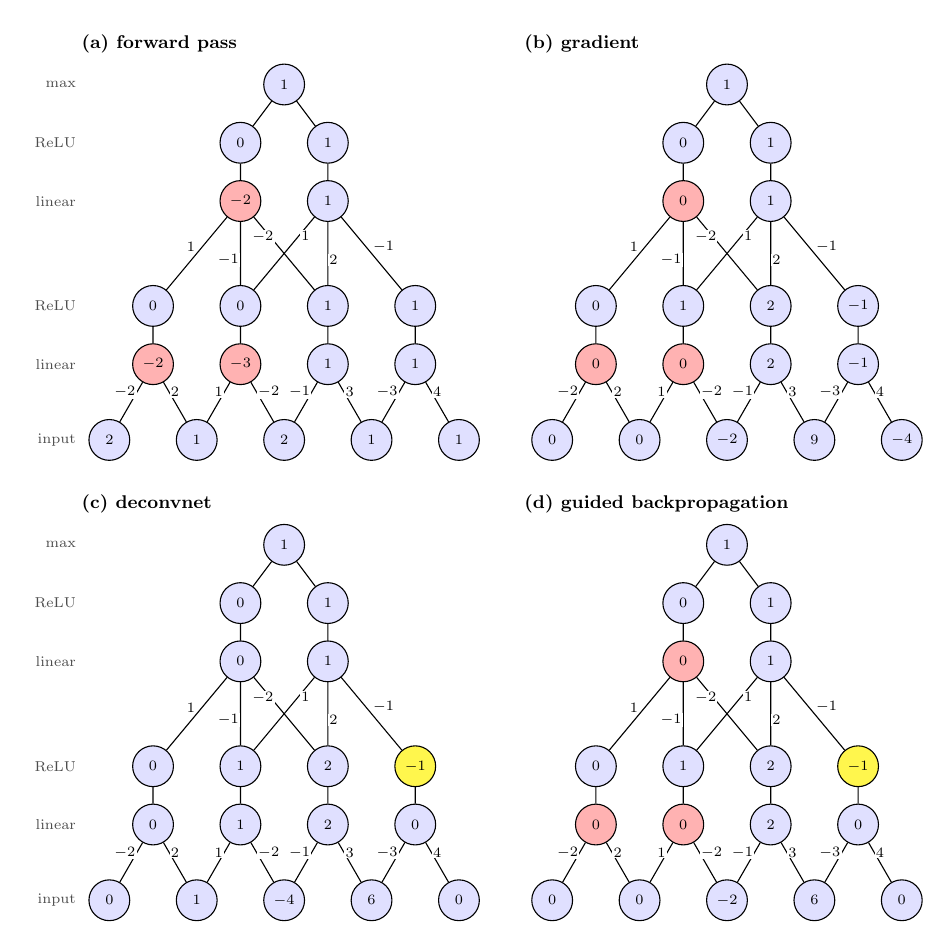
\begin{tikzpicture}[scale=0.74, every node/.append style={transform shape}, wlab/.append style={font=\scriptsize}]
    \begin{scope}
      \toycnn{2/nn,1/nn,2/nn,1/nn,1/nn}{-2/nnr,-3/nnr,1/nn,1/nn}{0/nn,0/nn,1/nn,1/nn}{-2/nnr,1/nn}{0/nn,1/nn}{1/nn}{(a) forward pass}
      \foreach \t/\y in {input/0, linear/1.3, ReLU/2.3, linear/4.1, ReLU/5.1, max/6.1} \node[lyr] at (-0.45,\y) {\t};
    \end{scope}
    \begin{scope}[xshift=7.6cm]
      \toycnn{0/nn,0/nn,-2/nn,9/nn,-4/nn}{0/nnr,0/nnr,2/nn,-1/nn}{0/nn,1/nn,2/nn,-1/nn}{0/nnr,1/nn}{0/nn,1/nn}{1/nn}{(b) gradient}
    \end{scope}
    \begin{scope}[yshift=-7.9cm]
      \toycnn{0/nn,1/nn,-4/nn,6/nn,0/nn}{0/nn,1/nn,2/nn,0/nn}{0/nn,1/nn,2/nn,-1/nny}{0/nn,1/nn}{0/nn,1/nn}{1/nn}{(c) deconvnet}
      \foreach \t/\y in {input/0, linear/1.3, ReLU/2.3, linear/4.1, ReLU/5.1, max/6.1} \node[lyr] at (-0.45,\y) {\t};
    \end{scope}
    \begin{scope}[xshift=7.6cm, yshift=-7.9cm]
      \toycnn{0/nn,0/nn,-2/nn,6/nn,0/nn}{0/nnr,0/nnr,2/nn,0/nn}{0/nn,1/nn,2/nn,-1/nny}{0/nnr,1/nn}{0/nn,1/nn}{1/nn}{(d) guided backpropagation}
    \end{scope}
  \end{tikzpicture}
  \caption{Backpropagation rules on a toy convolution-like network with zero intercepts. Edge labels are weights. (a) Forward pass for the input $\vx=(2,1,2,1,1)$; red nodes have negative pre-activations, so the ReLU above them outputs zero. (b)--(d) Backward passes; each node holds the backpropagated value for that node, starting from 1 at the output, and the bottom row is the score for each input. (b) The gradient zeroes the signal through ReLUs whose forward input was negative (red). (c) The deconvnet instead zeroes negative backward signals at each ReLU (yellow), ignoring the forward pass. (d) Guided backpropagation applies both rules.}
  \label{fig:toycnn}
\end{figure}

The backward pass (Figure~\ref{fig:toycnn}b) stores at each node the gradient of the output $y$ with respect to that node. It starts from $\partial y/\partial y=1$ at the output and applies the chain rule: if $u$ feeds into $v$, which feeds into $y$, then $\partial y/\partial u=\frac{\partial y}{\partial v}\frac{\partial v}{\partial u}$, summed over all such $v$. Three local derivatives are needed.
\begin{itemize}
  \item \emph{Max.} $y=\max(h_1^{(2)},h_2^{(2)})=\max(0,1)$. Changing the winning input $h^{(2)}_2=1$ by a small $\epsilon$ changes $y$ by $\epsilon$, while changing the losing input $h^{(2)}_1=0$ slightly does not change $y$ at all. So $\partial y/\partial h^{(2)}=(0,1)$: the max routes the gradient to its winning input, sometimes called the max ``switch''.
  \item \emph{ReLU.} $\partial h/\partial z=\ind[z>0]$: the gradient passes unchanged through a ReLU whose input was positive, on the sloped part of the function, and is zeroed where the input was negative, on the flat part. Since $\vz^{(2)}=(-2,1)$, $\partial y/\partial\vz^{(2)}=(0,1)$. This depends on the forward pass, which is why backpropagation must store the intermediate values computed in the forward pass and why it needs more memory than prediction alone.
  \item \emph{Linear.} For $\vz=\mW\vh$, $\partial z_j/\partial h_k=W_{jk}$, so $\partial y/\partial\vh=\mW^\top\,\partial y/\partial\vz$: the backward pass uses the same edge weights as the forward pass, in the opposite direction.
\end{itemize}
Continuing, $\partial y/\partial\vh^{(1)}=\mW^{(2)\top}(0,1)^\top=(0,1,2,-1)$. The ReLU zeroes the first two entries because $z^{(1)}_1,z^{(1)}_2<0$, giving $\partial y/\partial\vz^{(1)}=(0,0,2,-1)$. Finally
\begin{equation}
  \nabla_{\vx}y = \mW^{(1)\top}(0,0,2,-1)^\top = (0,\,0,\,-2,\,9,\,-4).
\end{equation}

\subsection{Gradient times input}

A common variant multiplies the gradient elementwise by the input, $s_i=x_i\,\partial f/\partial x_i$, which here gives $(0,0,-4,9,-4)$. The logic is that a feature equal to zero cannot have contributed to the output. This is somewhat arbitrary for continuous features, whose zero may have no special meaning. It is natural for one-hot DNA: $x_{b,l}$ is one for the observed base and zero otherwise, so gradient $\times$ input keeps only the gradient at the observed base of each position. Gradient $\times$ input, computed by ordinary (``vanilla'') backpropagation, is often itself called a saliency map. Note that the gradient is close to zero wherever the output is locally flat in $\vx$, even if a larger change in $\vx$ would change the output substantially; we return to this in Section~\ref{sec:failure_modes}.

In practice gradient-based saliency maps highlight the right regions, but are noisy: on simulated sequences in which the positive class requires two motifs, the gradient highlights both motifs but also many background positions~\citep{shrikumar2017}; we will reproduce this in Section~\ref{sec:sim_example}.

%======================================================================
\section[Deconvnets and guided backpropagation]{Modified backpropagation: deconvnets and guided backpropagation}
\label{sec:modified_backprop}
%======================================================================

Several methods keep the cost of one backward pass but change how the backward signal passes through the non-linearities. For ReLU networks with max pooling, the only non-linear steps are the ReLUs and the max switches, so each method is defined by its ReLU rule.

\subsection{Deconvolutional networks}

Deconvolutional networks were originally proposed for unsupervised learning and were adapted to visualize image classifiers by \citet{zeiler2014}. Applied to attribution, the ``deconvnet'' runs the network backwards like backpropagation, using the same weights and the same max switches, but treats each ReLU differently. Instead of zeroing the signal where the forward input to the ReLU was negative, it applies the ReLU to the backward signal itself, zeroing it wherever it is negative. On the toy network (Figure~\ref{fig:toycnn}c), the backward signal at the second ReLU is $(0,1)$ regardless of $\vz^{(2)}$, at the first ReLU the signal $(0,1,2,-1)$ becomes $(0,1,2,0)$, and the input scores are $\mW^{(1)\top}(0,1,2,0)^\top=(0,1,-4,6,0)$.

The deconvnet solves the computational problem in the same way as the gradient. It does not solve the saturation problem, and its output has no precise mathematical meaning: it is a heuristic that ``runs the ReLU backwards''. In examples it can look qualitatively different from the gradient, and somewhat less noisy, but it still highlights many unimportant positions.

\subsection{Guided backpropagation}

The gradient and the deconvnet each seem to have advantages, so guided backpropagation~\citep{springenberg2015} combines them: at each ReLU, the backward signal is zeroed both where the forward input was negative \emph{and} where the backward signal is negative. On the toy network (Figure~\ref{fig:toycnn}d) the first ReLU now sees $(0,1,2,-1)$, zeroes the first two entries because of the forward pass and the last because it is negative, giving $(0,0,2,0)$, and the input scores are $(0,0,-2,6,0)$. Guided backpropagation typically gives sparser, cleaner maps than either the gradient or the deconvnet.

Figure~\ref{fig:relu_rules} summarizes the three rules on a $3\times 3$ layer, as in an image. Let $z$ be the input to a ReLU in the forward pass and $g$ the backward signal arriving at its output. The signal passed back to $z$ is
\begin{equation}
  \text{gradient: } g\,\ind[z>0], \qquad \text{deconvnet: } \max(g,0), \qquad \text{guided: } \max(g,0)\,\ind[z>0].
  \label{eq:relu_rules}
\end{equation}

\begin{figure}[t]
  \centering
  \newcommand{\threebythree}[4]{% #1 values, #2 cells to colour red, #3 cells to colour yellow, #4 label
    \begin{scope}
      \foreach \v [count=\i from 0] in {#1} {
        \pgfmathtruncatemacro{\r}{\i/3}\pgfmathtruncatemacro{\c}{mod(\i,3)}
        \draw[fill=white] (\c*0.55,-\r*0.55) rectangle ++(0.55,-0.55);
      }
      \foreach \i in {#2} {\pgfmathtruncatemacro{\r}{\i/3}\pgfmathtruncatemacro{\c}{mod(\i,3)}
        \fill[red!30] (\c*0.55,-\r*0.55) rectangle ++(0.55,-0.55);}
      \foreach \i in {#3} {\pgfmathtruncatemacro{\r}{\i/3}\pgfmathtruncatemacro{\c}{mod(\i,3)}
        \fill[yellow!70] (\c*0.55,-\r*0.55) rectangle ++(0.55,-0.55);}
      \foreach \v [count=\i from 0] in {#1} {
        \pgfmathtruncatemacro{\r}{\i/3}\pgfmathtruncatemacro{\c}{mod(\i,3)}
        \draw (\c*0.55,-\r*0.55) rectangle ++(0.55,-0.55);
        \node[font=\scriptsize] at (\c*0.55+0.275,-\r*0.55-0.275) {$\v$};
      }
      \node[font=\footnotesize, above] at (0.825,0) {#4};
    \end{scope}}
  \begin{tikzpicture}[>=Stealth]
    \threebythree{3,-1,2,-2,1,-4,1,5,-3}{1,3,5,8}{}{ReLU input $z$}
    \draw[->] (1.8,-0.825) -- (3.0,-0.825) node[midway, above, font=\scriptsize] {forward};
    \begin{scope}[xshift=3.15cm]\threebythree{3,0,2,0,1,0,1,5,0}{}{}{output $\relu(z)$}\end{scope}
    \begin{scope}[xshift=6.6cm]\threebythree{1,-2,3,2,4,-1,-3,1,2}{}{1,5,6}{backward signal $g$}\end{scope}
    \begin{scope}[yshift=-2.6cm]
      \begin{scope}[xshift=0cm]\threebythree{1,0,3,0,4,0,-3,1,0}{1,3,5,8}{}{gradient}\end{scope}
      \begin{scope}[xshift=3.3cm]\threebythree{1,0,3,2,4,0,0,1,2}{}{1,5,6}{deconvnet}\end{scope}
      \begin{scope}[xshift=6.6cm]\threebythree{1,0,3,0,4,0,0,1,0}{1,3,5,8}{6}{guided backprop}\end{scope}
    \end{scope}
  \end{tikzpicture}
  \caption{The three ReLU rules on a $3\times 3$ layer. Top: the forward pass (red, $z<0$) and the backward signal arriving at the ReLU output (yellow, $g<0$). Bottom: the signal passed back to $z$. The gradient zeroes cells where the forward input was negative, the deconvnet zeroes cells where the backward signal is negative, and guided backpropagation zeroes both. Layout after \citet{springenberg2015}, with different numbers.}
  \label{fig:relu_rules}
\end{figure}

\subsection{Intuition: positive paths}

Guided backpropagation is a heuristic, but there is an intuitive argument for it~\citep{guerzhoy_video}. Since the network is linear apart from the ReLUs and max switches, the gradient with respect to an input is a sum over all paths from that input to the output of the product of the weights along the path, restricted to paths through active units. Some paths carry positive evidence and others negative evidence. Consider an image classifier that outputs the probability of ``cat'' (Figure~\ref{fig:positive_paths}). A pixel in the eye of a cat activates a ``cat eye'' unit, which is positive evidence for a cat. The same pixel may also feed, with a negative weight, into a ``dog ear'' unit that in turn provides evidence against a cat. The gradient adds the positive and negative paths, so that the pixel's importance is partly cancelled. Guided backpropagation only propagates signal along paths on which the backward signal stays positive. It therefore sums only positive evidence, which gives sparser maps in which the features that support the prediction stand out. The price is that it ignores negative evidence entirely.

\begin{figure}[t]
  \centering
  \begin{tikzpicture}[>=Stealth, every node/.style={font=\small}]
    \node[draw, ellipse, fill=gray!10] (cat) at (0,2.6) {cat?};
    \node[draw, ellipse, fill=gray!10] (eye) at (-2.2,1.2) {``cat eye'' unit};
    \node[draw, ellipse, fill=gray!10] (ear) at (2.2,1.2) {``dog ear'' unit};
    \node[draw, minimum size=6mm, fill=orange!30] (pix) at (0,-0.2) {};
    \node[below=1mm of pix] {pixel in the cat's eye};
    \draw[->, thick, green!50!black] (pix) -- node[left, font=\footnotesize] {$+$} (eye);
    \draw[->, thick, green!50!black] (eye) -- node[left, font=\footnotesize] {$+$} (cat);
    \draw[->, thick, red!70!black] (pix) -- node[right, font=\footnotesize] {$-$} (ear);
    \draw[->, thick, red!70!black] (ear) -- node[right, font=\footnotesize] {$-$} (cat);
    \node[red!70!black, font=\Large] at (1.2,1.85) {$\times$};
  \end{tikzpicture}
  \caption{Intuition for guided backpropagation. A pixel provides positive evidence for ``cat'' through a cat-eye detector (green path). The gradient also counts paths through other units, such as one through a dog-ear detector, which may carry signal of the opposite sign (red path). Guided backpropagation drops paths on which the backward signal becomes negative (cross). After an example by M.~Guerzhoy~\citep{guerzhoy_video}.}
  \label{fig:positive_paths}
\end{figure}

\subsection{Limitations}

These methods share several limitations.
\begin{itemize}
  \item They are defined for ReLUs (and max pooling). Modern networks use many other non-linearities, such as GELU, sigmoid and softmax, for which there is no obvious analogue of~\eqref{eq:relu_rules}.
  \item They ignore intercept terms, which, as we will see next, is part of why they fail on saturation and threshold effects.
  \item The deconvnet and guided backpropagation are not explanations of the model in any precise sense. Guided backpropagation in particular can produce plausible-looking maps that change little when the network's weights are randomized~\citep{adebayo2018}, because in deep image networks it largely reconstructs the input~\citep{nie2018}. Visual appeal is not evidence of faithfulness to the model.
\end{itemize}

\subsection{Saturation and thresholds revisited}
\label{sec:failure_modes}

Return to the saturating network~\eqref{eq:sat_net} at $\vx=(1,1)$. The backward signal at $h$ is the output weight, $\partial y/\partial h=-1$. The forward input to the ReLU is $z=-1<0$, so the gradient is zeroed; the deconvnet zeroes it because $-1<0$; and guided backpropagation zeroes it for both reasons. All three methods give scores $(0,0)$ for $x_1$ and $x_2$, the same failure as single-feature perturbation. The gradient describes the function at $\vx$, where it is flat, and says nothing about how the output got there.

\begin{figure}[t]
  \centering
  \newcommand{\thrnet}[9]{% inputs a,b,c ; za, ra ; zb, rb ; y ; title
    \node[nn] (a) at (0,0) {$#1$}; \node[nn] (b) at (1.4,0) {$#2$}; \node[nn] (c) at (2.8,0) {$#3$};
    \node[nn] (za) at (0,1.2) {$#4$}; \node[nn] (ra) at (0,2.2) {$#5$};
    \node[nn] (zb) at (2.1,1.2) {$#6$}; \node[nn] (rb) at (2.1,2.2) {$#7$};
    \node[nn] (y) at (1.05,3.3) {$#8$};
    \draw (a) -- node[wlab, left] {$1$} (za); \draw (za) -- (ra);
    \draw (b) -- node[wlab, left] {$1$} (zb); \draw (c) -- node[wlab, right] {$-1.5$} (zb); \draw (zb) -- (rb);
    \draw (ra) -- node[wlab, left] {$2$} (y); \draw (rb) -- node[wlab, right] {$2$} (y);
    \node[font=\footnotesize, below] at (a.south) {$a$}; \node[font=\footnotesize, below] at (b.south) {$b$};
    \node[font=\footnotesize, below] at (c.south) {$c$};
    \node[font=\small\bfseries, anchor=west] at (-0.5,4.0) {#9};}
  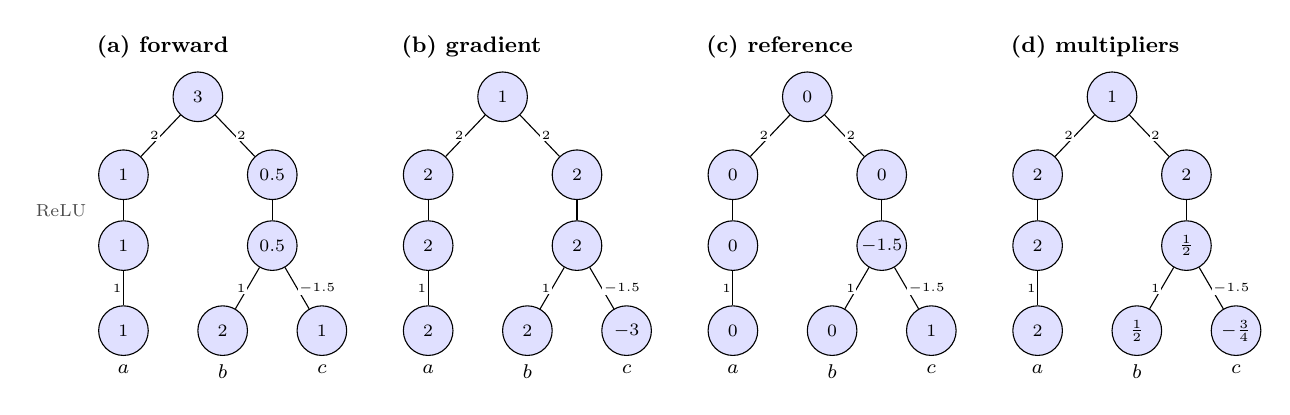
\begin{tikzpicture}[scale=0.9, every node/.append style={transform shape}]
    \thrnet{1}{2}{1}{1}{1}{0.5}{0.5}{3}{(a) forward}
    \node[lyr] at (-0.4,1.7) {ReLU};
    \begin{scope}[xshift=4.3cm]\thrnet{2}{2}{-3}{2}{2}{2}{2}{1}{(b) gradient}\end{scope}
    \begin{scope}[xshift=8.6cm]\thrnet{0}{0}{1}{0}{0}{-1.5}{0}{0}{(c) reference}\end{scope}
    \begin{scope}[xshift=12.9cm]\thrnet{2}{\frac12}{-\frac34}{2}{2}{\frac12}{2}{1}{(d) multipliers}\end{scope}
  \end{tikzpicture}
  \caption{The threshold failure mode. (a) A network with output $y=2\relu(a)+2\relu(b-1.5c)$ evaluated at $(a,b,c)=(1,2,1)$; the input $c$ acts as a fixed threshold. (b) Gradients: gradient $\times$ input gives $a$ a score of 2 and $b$ a score of 4, although the left branch contributes 2 to the output and the right branch only 1. (c) The reference input $(0,0,1)$, with output 0. (d) DeepLIFT multipliers $m_{\Delta u\Delta y}$ for each node $u$; contributions $m\,\Delta u$ are 2 for $a$, 1 for $b$ and 0 for $c$, summing to $\Delta y=3$ (Section~\ref{sec:deeplift}).}
  \label{fig:threshold}
\end{figure}

A second failure mode involves thresholds (Figure~\ref{fig:threshold}a). Consider three inputs $a,b,c$ and the network
\begin{equation}
  y = 2\,\relu(a) + 2\,\relu(b - 1.5\,c),
\end{equation}
where $c$ is held at 1, so that it acts as a threshold of 1.5 on $b$, like an intercept. At $(a,b,c)=(1,2,1)$, the left branch contributes $2\times 1=2$ to $y$ and the right branch $2\times 0.5=1$, so $y=3$. Both ReLUs are active, and the gradients are $\partial y/\partial a=2$, $\partial y/\partial b=2$ and $\partial y/\partial c=-3$ (Figure~\ref{fig:threshold}b). Gradient $\times$ input gives scores of $2\times1=2$ for $a$ and $2\times 2=4$ for $b$, ranking $b$ above $a$, although $a$ is responsible for more of the output. The gradient sees only the local slope of the right branch, not that most of $b$'s value is spent getting over the threshold.

%======================================================================
\section{DeepLIFT: differences from a reference}
\label{sec:deeplift}
%======================================================================

DeepLIFT~\citep{shrikumar2017} moves away from gradients. It explains the difference between the output for the input of interest and the output for a \emph{reference} input, and propagates these differences, rather than infinitesimal changes, back through the network. This solves the saturation and threshold problems, handles intercepts, and is defined for activation functions other than ReLU. It keeps the computational cost of a single backward pass.

\subsection{Contributions and multipliers}

Let $\vx^0\in\R^P$ be a reference input, with output $y^0=f(\vx^0)$. For every node $u$ of the network (an input, a hidden unit or the output) let $u^0$ be its value when the network is run on $\vx^0$, and $\Delta u=u-u^0$ its difference from reference. In particular $\Delta x_i=x_i-x^0_i$ and $\Delta y=y-y^0$. DeepLIFT assigns to each input a \emph{contribution} $C_{\Delta x_i\Delta y}\in\R$, the part of $\Delta y$ attributed to $\Delta x_i$, such that the contributions satisfy \emph{summation-to-delta},
\begin{equation}
  \sum_{i=1}^P C_{\Delta x_i\Delta y} = \Delta y .
  \label{eq:sum_to_delta}
\end{equation}
The \emph{multiplier} is the contribution per unit difference,
\begin{equation}
  m_{\Delta x_i\Delta y} = \frac{C_{\Delta x_i\Delta y}}{\Delta x_i}.
  \label{eq:multiplier}
\end{equation}
The multiplier is a finite-difference analogue of the partial derivative $\partial y/\partial x_i$, which is the limit of $\Delta y/\Delta x$ as $\Delta x\to 0$. In one dimension, the gradient is the slope of the tangent at $x$, while the multiplier is the slope of the secant from the reference $x^0$ to $x$ (Figure~\ref{fig:secant}). Where the function saturates, the tangent is flat but the secant is not.

\begin{figure}[t]
  \centering
  \includegraphics[width=0.55\linewidth]{secant.pdf}
  \caption{Gradient versus DeepLIFT multiplier for a sigmoid unit $\sigma(z)=1/(1+e^{-z})$, with reference $z^0=0$ (where $\sigma=0.5$) and input $z=4$. The gradient is the slope of the tangent at $z$ and is close to zero because the sigmoid has saturated. The multiplier is the slope of the secant from $z^0$ to $z$, $\Delta y/\Delta z$, and remains substantial. For $z\gg 0$ the difference from reference approaches $+0.5$.}
  \label{fig:secant}
\end{figure}

\subsection{The chain rule for multipliers}

Multipliers can be backpropagated in the same way as gradients. Recall the chain rule for gradients: if a parameter $w$ affects $y$ only through intermediate nodes $x_1,\dots,x_P$, then $\frac{\partial y}{\partial w}=\sum_i\frac{\partial x_i}{\partial w}\frac{\partial y}{\partial x_i}$. The analogous rule for multipliers is the following. Let $x_1,\dots,x_P$ be the inputs and $z_1,\dots,z_J$ a layer of nodes such that every path from the inputs to $y$ passes through exactly one $z_j$. Suppose we have multipliers $m_{\Delta x_i\Delta z_j}$ that satisfy summation-to-delta for each $z_j$, $\sum_i m_{\Delta x_i\Delta z_j}\Delta x_i=\Delta z_j$, and multipliers $m_{\Delta z_j\Delta y}$ that satisfy $\sum_j m_{\Delta z_j\Delta y}\Delta z_j=\Delta y$. Define
\begin{equation}
  m_{\Delta x_i\Delta y} = \sum_{j=1}^J m_{\Delta x_i\Delta z_j}\, m_{\Delta z_j\Delta y}.
  \label{eq:mult_chain}
\end{equation}
Then summation-to-delta holds for the composition, since
\begin{equation}
  \sum_{i=1}^P m_{\Delta x_i\Delta y}\Delta x_i
  = \sum_{j=1}^J m_{\Delta z_j\Delta y}\sum_{i=1}^P m_{\Delta x_i\Delta z_j}\Delta x_i
  = \sum_{j=1}^J m_{\Delta z_j\Delta y}\,\Delta z_j = \Delta y .
\end{equation}
Applying~\eqref{eq:mult_chain} layer by layer from the output down gives the multiplier of every node with respect to $y$ in one backward pass, after one forward pass on the input and one on the reference. We write $m_{\Delta u\Delta y}$ for the multiplier stored at node $u$, and $m_{\Delta u\Delta v}$ for the multiplier on an edge from $u$ to $v$, the analogue of $\partial v/\partial u$. Exactly as for gradients, the value at a node is the sum over its outgoing edges of the edge multiplier times the value at the node above.

\subsection{Rules for linear units and ReLUs}

We need local multipliers for each type of operation (Table~\ref{tab:mult_rules}).

\paragraph{Linear units.} For $z=b+\sum_i w_ix_i$ with intercept $b$, the reference value is $z^0=b+\sum_iw_ix_i^0$, so $\Delta z=\sum_i w_i\Delta x_i$: the intercept cancels. The natural contributions are $C_{\Delta x_i\Delta z}=w_i\Delta x_i$, which satisfy summation-to-delta, and the multipliers are $m_{\Delta x_i\Delta z}=w_i$, the same as the gradient.

\paragraph{ReLUs (the Rescale rule).} For $h=\relu(z)$, with a single input, summation-to-delta forces $C_{\Delta z\Delta h}=\Delta h$, so
\begin{equation}
  m_{\Delta z\Delta h} = \frac{\Delta h}{\Delta z} = \frac{\relu(z)-\relu(z^0)}{z-z^0}.
  \label{eq:rescale}
\end{equation}
When $\Delta z=0$ we also have $\Delta h=0$, and the multiplier is set to the gradient, its limit as $\Delta z\to 0$. The same rule applies to any elementwise non-linearity $h=\sigma(z)$, such as a sigmoid, tanh or GELU, by replacing $\relu$ with $\sigma$ in~\eqref{eq:rescale}. Unlike the gradient, the multiplier depends on the reference value $z^0$ as well as on $z$. \citet{shrikumar2017} also propose a ``RevealCancel'' rule, which treats positive and negative contributions to $\Delta z$ separately; we use only Rescale here.

\begin{table}[t]
  \centering
  \caption{Gradients and DeepLIFT multipliers for the two operations of a ReLU network. $\ind[\cdot]$ is the indicator function and $\Delta$ denotes the difference from the reference.}
  \label{tab:mult_rules}
  \begin{tabular}{lll}
    \toprule
    Function & Gradient & Multiplier \\
    \midrule
    $z=b+\sum_iw_ix_i$ & $\partial z/\partial x_i = w_i$ & $C_{\Delta x_i\Delta z}=w_i\Delta x_i$, \quad $m_{\Delta x_i\Delta z}=w_i$ \\[2pt]
    $h=\max(0,z)$ & $\partial h/\partial z=\ind[z>0]$ & $C_{\Delta z\Delta h}=\Delta h$, \quad $m_{\Delta z\Delta h}=\Delta h/\Delta z$ \\
    \bottomrule
  \end{tabular}
\end{table}

\subsection{Saturation and thresholds with DeepLIFT}

\begin{figure}[t]
  \centering
  \newcommand{\satnet}[6]{% x1, x2, z, h, y, title
    \node[nn] (x1) at (0,0) {$#1$}; \node[nn] (x2) at (1.4,0) {$#2$};
    \node[nn] (z) at (0.7,1.2) {$#3$}; \node[nn] (h) at (0.7,2.1) {$#4$}; \node[nn] (y) at (0.7,3.1) {$#5$};
    \node[nnb, right=1mm of z] {$+1$}; \node[nnb, right=1mm of y] {$+1$};
    \draw (x1) -- node[wlab, left] {$-1$} (z); \draw (x2) -- node[wlab, right] {$-1$} (z);
    \draw (z) -- (h); \draw (h) -- node[wlab, left] {$-1$} (y);
    \node[font=\footnotesize, below] at (x1.south) {$x_1$}; \node[font=\footnotesize, below] at (x2.south) {$x_2$};
    \node[font=\small\bfseries, anchor=west] at (-0.5,3.8) {#6};}
  \begin{tikzpicture}
    \satnet{1}{1}{-1}{0}{1}{(a) input}
    \node[lyr] at (0.35,1.65) {ReLU};
    \begin{scope}[xshift=3.6cm]\satnet{0}{0}{1}{1}{0}{(b) reference}\end{scope}
    \begin{scope}[xshift=7.2cm]\satnet{\frac12}{\frac12}{-\frac12}{-1}{1}{(c) multipliers}
      \node[font=\scriptsize, right] at (1.45,1.65) {$\dfrac{\Delta h}{\Delta z}=\dfrac{0-1}{-1-1}=\dfrac12$};
      \node[font=\footnotesize, below=0.35cm] at (x1.south) {$C=\frac12$};
      \node[font=\footnotesize, below=0.35cm] at (x2.south) {$C=\frac12$};
    \end{scope}
  \end{tikzpicture}
  \caption{DeepLIFT on the saturating network of Figure~\ref{fig:saturation}. (a) Forward pass on the input $(1,1)$. (b) Forward pass on the reference $(0,0)$. (c) Backward pass of multipliers $m_{\Delta u\Delta y}$, starting from 1 at the output. The ReLU multiplier is $\Delta h/\Delta z=\frac12$, so each input receives multiplier $\frac12$ and contribution $C=m\,\Delta x=\frac12$; the contributions sum to $\Delta y=1$.}
  \label{fig:deeplift_sat}
\end{figure}

For the saturating network~\eqref{eq:sat_net}, take the reference $\vx^0=(0,0)$ (Figure~\ref{fig:deeplift_sat}). On the reference, $z^0=1$, $h^0=1$ and $y^0=0$; on the input $(1,1)$, $z=-1$, $h=0$ and $y=1$, so $\Delta y=1$. Backpropagating multipliers: the output node has multiplier 1; the edge from $h$ to $y$ is linear with weight $-1$, so $m_{\Delta h\Delta y}=-1$. The ReLU multiplier is $\Delta h/\Delta z=(0-1)/(-1-1)=\frac12$, where the gradient would be 0, so $m_{\Delta z\Delta y}=-1\times\frac12=-\frac12$. Each input edge has weight $-1$, so $m_{\Delta x_1\Delta y}=m_{\Delta x_2\Delta y}=\frac12$, and the contributions are $C_{\Delta x_i\Delta y}=\frac12\times 1=\frac12$. Both inputs receive equal credit, and the contributions sum to $\Delta y=1$. The gradient was zero because the output is flat at $\vx$; the multiplier sees the whole change from the reference.

For the threshold network (Figure~\ref{fig:threshold}c,d), take the reference $(a,b,c)=(0,0,1)$, which keeps the threshold input $c$ at its value. The reference output is $y^0=2\relu(0)+2\relu(-1.5)=0$, so $\Delta y=3$. In the left branch, the ReLU multiplier is $(1-0)/(1-0)=1$, so $m_{\Delta a\Delta y}=2$ and $C_{\Delta a\Delta y}=2\times 1=2$. In the right branch, the pre-activation goes from $-1.5$ to $0.5$ and the activation from $0$ to $0.5$, so the ReLU multiplier is $0.5/2=\frac14$, $m_{\Delta b\Delta y}=2\times\frac14\times 1=\frac12$ and $C_{\Delta b\Delta y}=\frac12\times 2=1$. Since $\Delta c=0$, $C_{\Delta c\Delta y}=0$. DeepLIFT therefore assigns 2 to $a$ and 1 to $b$, matching the amounts each branch adds to the output, where gradient $\times$ input gave 2 and 4.

\subsection{A worked example}
\label{sec:deeplift_example}

Consider a network with four inputs $\vx\in\R^4$, three hidden ReLU units with intercepts, and a linear output with no intercept,
\begin{equation}
  \begin{aligned}
    z_1 &= 2x_1 + x_2 - 1, & z_2 &= -x_2 + x_3, & z_3 &= -2x_3 + 2x_4 + 2,\\
    y &= -\relu(z_1) + 2\relu(z_2) + \relu(z_3). & & & &
  \end{aligned}
  \label{eq:ex1_net}
\end{equation}
At the input $\vx=(1,2,0,1)$ the pre-activations are $\vz=(3,-2,4)$, the activations $\vh=(3,0,4)$ and the output $y=-3+0+4=1$. At the reference $\vx^0=\mathbf{0}$ they are $\vz^0=(-1,0,2)$, $\vh^0=(0,0,2)$ and $y^0=2$, so $\Delta y=-1$. The multipliers of the activations are the output weights, $(-1,2,1)$. The ReLU multipliers are
\begin{equation}
  \frac{\Delta h_1}{\Delta z_1}=\frac{3-0}{3-(-1)}=\frac34, \qquad
  \frac{\Delta h_2}{\Delta z_2}=\frac{0-0}{-2-0}=0, \qquad
  \frac{\Delta h_3}{\Delta z_3}=\frac{4-2}{4-2}=1,
\end{equation}
so the multipliers of the pre-activations are $(-1\times\frac34,\;2\times 0,\;1\times 1)=(-\frac34,0,1)$. Each input multiplier is the sum over its outgoing edges of weight times the multiplier above, for example $m_{\Delta x_2\Delta y}=1\times(-\frac34)+(-1)\times 0=-\frac34$. Table~\ref{tab:deeplift_example} collects the results and compares them with the gradient. The DeepLIFT contributions sum to $\Delta y=-1$; gradient $\times$ input sums to $-2$, because the gradient ignores the intercepts and the change in the third ReLU's operating point between reference and input.

\begin{table}[t]
  \centering
  \caption{Gradient and DeepLIFT for the network~\eqref{eq:ex1_net} at $\vx=(1,2,0,1)$ with reference $\vx^0=\mathbf{0}$. The DeepLIFT contributions sum to $\Delta y=y-y^0=1-2=-1$.}
  \label{tab:deeplift_example}
  \begin{tabular}{crrrrr}
    \toprule
    Input & $\Delta x_i$ & $\partial y/\partial x_i$ & $x_i\,\partial y/\partial x_i$ & $m_{\Delta x_i\Delta y}$ & $C_{\Delta x_i\Delta y}$ \\
    \midrule
    $x_1$ & 1 & $-2$ & $-2$ & $-\frac32$ & $-\frac32$ \\[1pt]
    $x_2$ & 2 & $-1$ & $-2$ & $-\frac34$ & $-\frac32$ \\[1pt]
    $x_3$ & 0 & $-2$ & 0 & $-2$ & 0 \\
    $x_4$ & 1 & 2 & 2 & 2 & 2 \\
    \midrule
    sum & & & $-2$ & & $-1$ \\
    \bottomrule
  \end{tabular}
\end{table}

\subsection{Relation to gradient times input}

If every intercept in a ReLU network is zero and the reference is $\vx^0=\mathbf{0}$, then every node has reference value zero. For a ReLU with $z>0$ the Rescale multiplier is $(z-0)/(z-0)=1$, and with $z<0$ it is $(0-0)/(z-0)=0$; both equal the gradient $\ind[z>0]$. Linear multipliers always equal the weights. Hence every multiplier equals the corresponding partial derivative, and the DeepLIFT contributions are $C_{\Delta x_i\Delta y}=x_i\,\partial y/\partial x_i$, gradient $\times$ input~\citep{shrikumar2017,ancona2018}. In this case gradient $\times$ input also sums to $y-y^0=y$: such a network is positively homogeneous, $f(\lambda\vx)=\lambda f(\vx)$ for $\lambda>0$, and differentiating with respect to $\lambda$ at $\lambda=1$ gives Euler's identity $\sum_i x_i\,\partial f/\partial x_i=f(\vx)$. The differences between the methods arise from the intercepts and from non-zero references, which is where gradient $\times$ input goes wrong in the examples above.

\subsection{Choosing the reference}

DeepLIFT scores answer the question ``important relative to what?'', and the answer depends on the reference. For images an all-black image is a common choice. For one-hot DNA, options include the all-zero input (no base at any position), the expected one-hot vector under background base frequencies (for example $0.25$ for each base), and shuffled versions of the input sequence that preserve its dinucleotide composition, with contributions averaged over several shuffles. A reference should be uninformative for the prediction, so that $\Delta y$ reflects the signal in the input. Figure~\ref{fig:secant} shows a related subtlety for sigmoid units: with reference pre-activation 0 the reference activation is $0.5$, not 0, and the difference from reference can be at most $0.5$ in either direction.

%======================================================================
\section{Integrated gradients}
\label{sec:ig}
%======================================================================

Integrated gradients~\citep{sundararajan2017} also explain $f(\vx)-f(\vx^0)$ relative to a reference (called the baseline), but use only gradients of $f$, with no special backpropagation rules. The idea is to average the gradient along the straight path from the reference to the input. Let $\boldsymbol{\gamma}(\alpha)=\vx^0+\alpha(\vx-\vx^0)$ for $\alpha\in[0,1]$. The integrated gradient of feature $i$ is
\begin{equation}
  \IG_i(\vx) = (x_i-x_i^0)\int_0^1 \frac{\partial f}{\partial x_i}\big(\boldsymbol{\gamma}(\alpha)\big)\,d\alpha .
  \label{eq:ig}
\end{equation}
Integrated gradients satisfy summation-to-delta, which \citet{sundararajan2017} call \emph{completeness}. By the fundamental theorem of calculus and the chain rule,
\begin{equation}
  f(\vx)-f(\vx^0) = \int_0^1 \frac{d}{d\alpha}f\big(\boldsymbol{\gamma}(\alpha)\big)\,d\alpha
  = \int_0^1 \sum_{i=1}^P \frac{\partial f}{\partial x_i}\big(\boldsymbol{\gamma}(\alpha)\big)\,(x_i-x_i^0)\,d\alpha
  = \sum_{i=1}^P \IG_i(\vx),
\end{equation}
using $d\gamma_i/d\alpha=x_i-x_i^0$. This requires $f$ to be differentiable almost everywhere along the path, which holds for ReLU networks.

\paragraph{The saturation example.} For $y=\min(x_1+x_2,1)$ with $\vx=(1,1)$ and $\vx^0=(0,0)$, the path is $\boldsymbol{\gamma}(\alpha)=(\alpha,\alpha)$, on which $y=\min(2\alpha,1)$. The gradient $\partial y/\partial x_1$ is 1 for $\alpha<\frac12$, before the function saturates, and 0 afterwards (Figure~\ref{fig:ig_sat}). The integral is $\frac12$, so $\IG_1=\IG_2=(1-0)\times\frac12=\frac12$, the same as DeepLIFT. For the threshold example, the gradient with respect to $a$ is 2 along the whole path, giving $\IG_a=2$. The right ReLU becomes active when $2\alpha-1.5>0$, that is for $\alpha>\frac34$, so $\IG_b=2\times\int_{3/4}^1 2\,d\alpha=1$, again matching DeepLIFT.

\begin{figure}[t]
  \centering
  \includegraphics[width=0.6\linewidth]{ig_saturation.pdf}
  \caption{Integrated gradients for $y=\min(x_1+x_2,1)$ along the path $\alpha\vx$ from the reference $(0,0)$ to $\vx=(1,1)$. The output (blue) rises until $\alpha=\frac12$ and then saturates, and the gradient with respect to $x_1$ (red) drops to zero. Its integral, the shaded area, is $\frac12$, so each input receives $\IG_i=\frac12$. Points mark a six-point Riemann approximation at $\alpha=0,0.2,\dots,1$, whose average is also $\frac12$.}
  \label{fig:ig_sat}
\end{figure}

\paragraph{Computation.} In practice the integral is approximated by a Riemann sum over $K$ points on the path (Algorithm~\ref{alg:ig}), typically with $K$ between 20 and 300, which costs $K$ gradient evaluations. In the saturation example, the gradient at $\alpha=0,0.2,0.4$ is 1 and at $\alpha=0.6,0.8,1$ is 0, whose average is $\frac12$, giving the same answer.

\begin{algorithm}[t]
  \caption{Integrated gradients with a midpoint Riemann sum}
  \label{alg:ig}
  \begin{algorithmic}[1]
    \Require model $f$, input $\vx$, reference $\vx^0$, number of steps $K$
    \State $\vg\gets\mathbf{0}\in\R^P$
    \For{$k=1,\dots,K$}
      \State $\alpha\gets (k-\frac12)/K$
      \State $\vg\gets\vg+\nabla_{\vx}f\big(\vx^0+\alpha(\vx-\vx^0)\big)$ \Comment{one forward and one backward pass}
    \EndFor
    \State \Return $(\vx-\vx^0)\odot\vg/K$ \Comment{$\odot$: elementwise product}
  \end{algorithmic}
\end{algorithm}

\paragraph{Pros and cons.} Integrated gradients treat the model as a black box apart from requiring its gradients, so they apply to any differentiable architecture. Because they depend only on the function $f$, two networks that compute the same function are guaranteed to receive the same attributions, a property called \emph{implementation invariance}. DeepLIFT's rules, in contrast, are applied to the network's computation graph, and two implementations of the same function can receive different DeepLIFT scores. The cost is the $K$ repeated gradient calculations, compared with one backward pass for DeepLIFT.

\paragraph{Expected gradients.} The choice of reference matters for integrated gradients as it does for DeepLIFT. \emph{Expected gradients}~\citep{erion2021} average integrated gradients over references drawn from the data, $\vx^0\sim\mathcal{D}$, and over the path position $\alpha\sim\mathrm{Uniform}(0,1)$,
\begin{equation}
  \mathrm{EG}_i(\vx) = \E_{\vx^0\sim\mathcal{D},\,\alpha\sim U(0,1)}\left[(x_i-x_i^0)\,\frac{\partial f}{\partial x_i}\big(\vx^0+\alpha(\vx-\vx^0)\big)\right],
\end{equation}
which is estimated by sampling pairs $(\vx^0,\alpha)$. This removes the need to pick a single reference and fits naturally into training with stochastic gradients.

%======================================================================
\section{Shapley values and SHAP}
\label{sec:shap}
%======================================================================

DeepLIFT and integrated gradients both distribute $f(\vx)-f(\vx^0)$ among the input features, but by different rules. Is there a principled way to choose among such rules? \citet{lundberg2017} showed that a small set of desirable properties singles out one attribution, based on the Shapley value from cooperative game theory~\citep{shapley1953}, and that several existing methods, DeepLIFT among them, can be viewed as approximations to it.

\subsection{Additive feature attribution}

Let $y=f(\vx)$ be the trained model. The goal is to find a simple explanation model $g\approx f$ that is valid near $\vx$. Explanations are defined on a \emph{simplified} binary input $\vx'\in\{0,1\}^P$ indicating which features are ``present'', together with a mapping $h_{\vx}$ back to the original input space. For DeepLIFT-style explanations, an absent feature takes its reference value,
\begin{equation}
  h_{\vx}(\vz')_i = \begin{cases} x_i^0 & \text{if } z'_i=0,\\ x_i & \text{if } z'_i=1,\end{cases}
\end{equation}
for $\vz'\in\{0,1\}^P$, so that $h_{\vx}(\mathbf{1})=\vx$ and $h_{\vx}(\mathbf{0})=\vx^0$. The input itself corresponds to $\vx'=\mathbf{1}$. An \emph{additive feature attribution} method uses an explanation model that is linear in the simplified inputs,
\begin{equation}
  g(\vz') = \phi_0 + \sum_{i=1}^P\phi_i z'_i ,
  \label{eq:additive}
\end{equation}
for $\vz'$ ``near'' $\vx'$, meaning $\vz'\subseteq\vx'$: $\vz'$ can only switch off features that are present in $\vx'$. Here $\phi_i\in\R$ is the attribution of feature $i$ and $\phi_0$ a constant. DeepLIFT is of this form, with $\phi_0=f(\vx^0)$ and $\phi_i=C_{\Delta x_i\Delta y}$, and so are integrated gradients, LIME and others.

\subsection{Three properties}

Write $f_{\vx}(\vz')=f(h_{\vx}(\vz'))$ for the model evaluated with only the features in $\vz'$ present, and $\vz'\setminus i$ for $\vz'$ with $z'_i$ set to zero. \citet{lundberg2017} ask for three properties.
\begin{enumerate}
  \item \emph{Local accuracy.} The explanation matches the model at the input: $f(\vx)=g(\vx')=\phi_0+\sum_i\phi_i x'_i$. With $\vx'=\mathbf{1}$ and $\phi_0=f(\vx^0)$ this is summation-to-delta.
  \item \emph{Missingness.} A feature that is absent gets no attribution: $x'_i=0\Rightarrow\phi_i=0$.
  \item \emph{Consistency.} If a model changes so that feature $i$'s marginal contribution never decreases, its attribution should not decrease. Formally, for two models $f$ and $\tilde f$, if
  \begin{equation}
    \tilde f_{\vx}(\vz')-\tilde f_{\vx}(\vz'\setminus i) \geq f_{\vx}(\vz')-f_{\vx}(\vz'\setminus i) \quad\text{for all } \vz'\in\{0,1\}^P,
  \end{equation}
  then $\phi_i(\tilde f,\vx)\geq\phi_i(f,\vx)$.
\end{enumerate}

\subsection{The Shapley value}

The theorem of \citet{lundberg2017}, building on classical results for the Shapley value, is that exactly one additive feature attribution satisfies all three properties. Treating the features as players in a cooperative game whose payoff for a coalition $S\subseteq\{1,\dots,P\}$ of present features is $f_{\vx}(S)$ (the model with features in $S$ at their input values and the rest at the reference), the attributions are the Shapley values
\begin{equation}
  \phi_i = \sum_{S\subseteq\{1,\dots,P\}\setminus\{i\}} \frac{|S|!\,(P-|S|-1)!}{P!}\Big[f_{\vx}(S\cup\{i\})-f_{\vx}(S)\Big].
  \label{eq:shapley}
\end{equation}
The bracket is the marginal contribution of feature $i$ when it is added to the features in $S$: how important $i$ is when the features in $S$ are on. The weight can be written $\frac{1}{P}\binom{P-1}{|S|}^{-1}$: it averages first over the $P$ possible sizes of $S$ and then over all subsets of a given size. Equivalently, $\phi_i$ is the average, over all $P!$ orderings in which the features could be switched on one at a time starting from the reference, of the change in output when feature $i$ is switched on.

For the saturation example with reference $\mathbf{0}$, $f_{\vx}(\emptyset)=0$ and $f_{\vx}(\{1\})=f_{\vx}(\{2\})=f_{\vx}(\{1,2\})=1$, so
\begin{equation}
  \phi_1 = \tfrac12\big[f_{\vx}(\{1\})-f_{\vx}(\emptyset)\big]+\tfrac12\big[f_{\vx}(\{1,2\})-f_{\vx}(\{2\})\big] = \tfrac12(1-0)+\tfrac12(1-1) = \tfrac12,
\end{equation}
and by symmetry $\phi_2=\frac12$. For the threshold example (treating $c$ as fixed), $f_{\vx}(\emptyset)=0$, $f_{\vx}(\{a\})=2$, $f_{\vx}(\{b\})=1$ and $f_{\vx}(\{a,b\})=3$, giving $\phi_a=\frac12(2+2)=2$ and $\phi_b=\frac12(1+1)=1$. In both examples the Shapley values coincide with the DeepLIFT and integrated gradients attributions. For a linear model $f(\vx)=b+\vw^\top\vx$ all three methods give $\phi_i=w_i(x_i-x_i^0)$. In general they differ (Exercise 5).

\subsection{Approximating Shapley values}

The sum~\eqref{eq:shapley} has $2^{P-1}$ terms for each feature, which is infeasible for a sequence model with $P=4L$ inputs. There are two broad options.
\begin{enumerate}
  \item \emph{Sampling.} Estimate~\eqref{eq:shapley} by Monte Carlo, sampling orderings or subsets $S$. KernelSHAP~\citep{lundberg2017} is a model-agnostic variant that fits the additive model~\eqref{eq:additive} by weighted linear regression to the model's outputs on sampled coalitions, with weights chosen so that the solution recovers the Shapley values. This resembles LIME with a particular choice of weights.
  \item \emph{Exploiting the structure of $f$.} For a linear model the Shapley values are available in closed form, and DeepLIFT's rules can be viewed as composing exact attributions of simple components through the chain rule~\eqref{eq:mult_chain}. DeepSHAP~\citep{lundberg2017} uses this view, running DeepLIFT with multipliers averaged over a distribution of references, and gives a fast approximation to Shapley values for deep networks.
\end{enumerate}
The SHAP framework thus provides a theoretical motivation for DeepLIFT-style methods: they are cheap approximations to the unique attribution that satisfies local accuracy, missingness and consistency.

%======================================================================
\section{Example: motifs in simulated regulatory sequence}
\label{sec:sim_example}
%======================================================================

To compare the methods on a problem where the ground truth is known, we follow the design of a simulation used to motivate DeepLIFT~\citep{shrikumar2017}. Random DNA sequences of length $L=200$ are generated with each base drawn uniformly. Two motifs are inserted at random non-overlapping positions: a GATA motif (consensus \texttt{AGATAAG}) and a TAL1-like E-box motif (consensus \texttt{AACAGATGGT}), each base matching the consensus with probability 0.95. A sequence is positive if it contains \emph{both} motifs; negatives contain only the GATA motif, only the TAL1 motif or neither, in equal proportions, so the model must learn an AND of the two motifs. We trained a small CNN on 10,000 sequences: one convolutional layer with 16 filters of width 11, a ReLU, global average pooling, a dense layer of 16 ReLU units and a single output logit. It reached an AUROC of 0.97 on 1,000 held-out sequences.

Figure~\ref{fig:seq_attr} shows six attribution maps for one correctly predicted positive sequence. DeepLIFT and integrated gradients use the reference that has probability $0.25$ for every base at every position. The observations are typical of what is seen in practice.
\begin{itemize}
  \item ISM, with 600 forward passes, gives a clean map: mutating any base in either motif lowers the prediction, and background positions have little effect.
  \item Gradient $\times$ input highlights both motifs, but its scores are noisier, include positions outside the motifs, and contain a large negative score inside the TAL1 motif.
  \item Guided backpropagation is almost identical to the gradient for this model. With global average pooling, the backward signal reaching each convolutional filter is the same at every position, and for the filters that are active here it is already positive, so the guided rule rarely zeroes anything.
  \item The deconvnet fails completely: it ignores whether each filter was active at each position, and so returns essentially the same combination of filter weights at every position, independent of where the motifs are. This illustrates the warning of Section~\ref{sec:modified_backprop} that modified backpropagation rules need not explain the model.
  \item DeepLIFT and integrated gradients closely resemble ISM. The DeepLIFT contributions sum exactly to the difference in logits between input and reference, $8.65$; integrated gradients with 500 steps sum to $8.74$, within 1\% of it, the residual being Riemann approximation error; gradient $\times$ input sums to $5.94$.
\end{itemize}

\begin{figure}[p]
  \centering
  \includegraphics[width=0.8\linewidth]{sequence_attributions.pdf}
  \caption{Attribution maps for a simulated positive sequence containing a TAL1-like motif (grey band at positions 72--81) and a GATA motif (grey band at 135--141), for a CNN trained to detect sequences containing both motifs. Each bar is the score of the observed base at that position, coloured by base and scaled so that the largest absolute score in each panel is 1. ISM is the mean decrease in the logit over the three possible mutations. DeepLIFT and integrated gradients use a uniform reference (probability 0.25 for each base) and are summed over the four bases at each position. Simulated data; see \texttt{scripts/make\_figures.py}.}
  \label{fig:seq_attr}
\end{figure}

For real genomic models, attribution maps computed for many sequences are the starting point for further analysis. High-scoring subsequences can be clustered to discover motifs, positions with large attributions can be compared with experimentally measured effects of mutations, and the effects of genetic variants can be predicted with ISM or approximated with gradients or DeepLIFT (Chapter 3).

%======================================================================
\section{Summary}
%======================================================================

\begin{itemize}
  \item Interpretation methods assign importance scores to input features, usually for one prediction at a time. For sequence models, the scores show which nucleotides drive a prediction and often reveal transcription factor motifs.
  \item In silico mutagenesis perturbs each feature and reruns the model. It is simple and directly predicts the effects of mutations, but it needs one forward pass per perturbation and misses features that matter only in combination (saturation).
  \item Backpropagation gives the gradient of the output with respect to every input in one backward pass, a local linear approximation of the model. Guided backpropagation and deconvnets change the ReLU rule to give cleaner maps, but are heuristics and share the gradient's failures on saturation and thresholds.
  \item DeepLIFT and integrated gradients explain the difference in output from a reference input and satisfy summation-to-delta (completeness), which solves the saturation problem. DeepLIFT backpropagates multipliers $\Delta\text{out}/\Delta\text{in}$ in one pass; integrated gradients average gradients along a path at the cost of many passes but depend only on the function.
  \item Shapley values are the unique additive attribution with local accuracy, missingness and consistency. They are exponentially expensive to compute exactly, and SHAP provides a framework in which DeepLIFT-type methods are fast approximations.
\end{itemize}

%======================================================================
\section*{Exercises}
%======================================================================

\begin{enumerate}
  \item The toy network of Figure~\ref{fig:toycnn} is changed in two ways: the first layer becomes $z^{(1)}_1=-x_1+2x_2$, $z^{(1)}_2=x_2+x_3$, $z^{(1)}_3=-x_3+3x_4$, $z^{(1)}_4=-3x_4+4x_5$, and the final max is replaced by the linear output $y=2h^{(2)}_1-h^{(2)}_2$; $\mW^{(2)}$ is unchanged. For the input $\vx=(0,2,1,0,3)$, compute the forward pass and the input scores given by the gradient, the deconvnet and guided backpropagation, and the corresponding saliency maps (scores $\times$ input). \emph{(Answer: $y=2$; gradient $(-2,2,-2,0,0)$; deconvnet and guided backpropagation both $(-2,4,0,0,0)$.)}
  \item A network has inputs $\vx\in\R^4$, pre-activations $z_1=x_1-x_2+2$, $z_2=2x_2+x_3-2$, $z_3=x_3-3x_4$, ReLU activations $h_j=\relu(z_j)$ and output $y=h_1-2h_2+2h_3$. For the input $\vx=(0,1,2,1)$ and reference $\vx^0=\mathbf{0}$, run the forward pass on both, label every node with its DeepLIFT multiplier, and compute the contributions of the four inputs. Check that they sum to $\Delta y$. \emph{(Answer: contributions $(0,-3,-2,0)$, $\Delta y=-3-2=-5$.)} Compare with gradient $\times$ input.
  \item Show that for a linear model $f(\vx)=b+\vw^\top\vx$, gradient $\times$ input (with $\vx-\vx^0$ in place of $\vx$), DeepLIFT, integrated gradients and Shapley values all give $\phi_i=w_i(x_i-x_i^0)$.
  \item Show that for a single unit $y=\sigma(\vw^\top\vx+b)$, where $\sigma$ is any differentiable non-linearity, the DeepLIFT Rescale contributions equal $w_i\Delta x_i\,\Delta y/\Delta z$ with $z=\vw^\top\vx+b$. Show that integrated gradients give the same attributions. (Hint: along the straight path, $z$ changes linearly in $\alpha$.)
  \item Consider $y=\relu(x_1+x_2-1)$ with reference $\mathbf{0}$ and input $\vx=(2,0.5)$. Compute the DeepLIFT, integrated gradients and Shapley attributions. \emph{(Answer: DeepLIFT and integrated gradients give $(1.2,0.3)$; Shapley values are $(1.25,0.25)$.)} Which do you find more reasonable, and why?
  \item Show that the gradient $\times$ input of a ReLU network with zero intercepts sums to $f(\vx)$. Give an example of a network with non-zero intercepts for which it does not sum to $f(\vx)-f(\mathbf{0})$.
  \item Using a trained sequence model, for example the simulation of Section~\ref{sec:sim_example}, compare ISM with the first-order approximation~\eqref{eq:ism_approx} across all positions and alternative bases. Where is the approximation worst?
\end{enumerate}
